\chapter[Software]{Software}
    
    \section[Sistema De Compras]{Sistema De Compras}
    
    \section[Sistema de Validação de Compra]{Sistema de Validação de Compra}
        
        O sistema de validação se trata do módulo responsável pela validação dos dados da compra,
        e dar o inicio no processo de serventia de chopp conforme as característias são pré-definidas.
        Esse subsistema tinha como resultados esperados uma aplicação que pudesse prover ao usuário
        a leitura do \textit{QRCode} gerado no momento da compra do chopp por meio de uma câmera 
        acoplada na máquina de onde o chopp é armazenado. No \textit{QRCode} estão contidas as informações
        referentes as preferências do consumidor no que tange sua bebida.
        
        Devido à necessidade de que o usuário tenha acesso a uma câmera para leitura do \textit{QRCode},
        foi escolhido o \textit{framework} Python Kivy\footnote{\url{https://kivy.org/}} por fornecer um ambiente
        \textit{touchscreen} com um baixo consumo de recursos, uma vez que essa aplicação estará 
        instanciada em uma Raspberry responsável por gerenciar outros módulos operacionais do projeto.

        Desta forma, foi então desenvolvida aplicação Autochopp-Machine \footnote{\url{https://github.com/autochopp/autochopp-machine}} que fornece de forma interativa 
        com a validação de \textit{QRCodes} e iniciação do processo de retirada do chopp. 

        Além do que foi citado, a aplicação também possui a responsabilidade de fazer requisições junto a API
        para que a mesma possa informar se o \textit{QRCode} lido é válido, significando que a compra foi 
        efetuada com sucesso, caso não śeja válido, é exibida uma mensagem de erro. A partir da combinação
        de preferências feitas no momento da compra, é gerado um identificador que é vinculado ao 
        \textit{QRCode}. Esse identificador é o responsável por passar as informações via socket para que
        os componentes eletrônicos vinculados a máquina sejam capazes de atuar na composição do chopp conforme
        suas especificações.

        \begin{figure}[H]
            \centering
            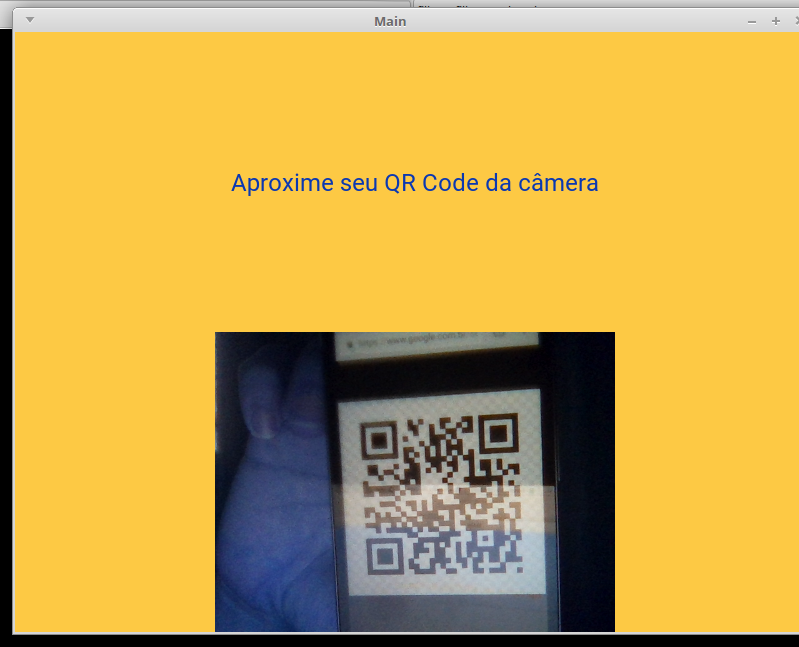
\includegraphics[scale= 0.4]{figuras/leitor-qrcode.png}
            \caption{Tela de Leitura de \textit{QRCode}. Fonte: Própria.}
            \label{leitor-qrcode}
        \end{figure}
